\section{Mapa de Navegación}

El mapa de navegación resume la arquitectura de información y los flujos de usuario de Argos. Conecta las pantallas de los mockups y define las rutas por rol para garantizar una navegación coherente e intuitiva.

\begin{samepage}\small\setlength{\parskip}{0.25\baselineskip}
\begin{figure}[H]
	\centering
	% Intentar cargar el diagrama; si no existe, mostrar un placeholder informativo de igual ancho
	\IfFileExists{./Media/MapaNavegacionpng.png}{%
		\includegraphics[width=1\textwidth]{./Media/MapaNavegacionpng.png}%
	}{%
		\IfFileExists{MapaNavegacionpng.png}{%
			\includegraphics[width=1\textwidth]{MapaNavegacionpng.png}%
		}{%
			\fbox{\parbox{0.98\textwidth}{\centering Imagen MapaNavegacionpng.png no disponible\\Coloque el archivo en ./Media/ o junto a este archivo}}% % chktex 26
		}%
	}
	\caption{Mapa de navegación de Argos por roles.}\label{fig:mapa-navegacion}
\end{figure}

\subsubsection*{Análisis del Flujo de Navegación}
\vspace{0.2\baselineskip}
Estructura jerárquica y ramificada:

\noindent \textbf{Inicio y Acceso.} Tras una posible pantalla de carga, el usuario llega a \textbf{Selección de Rol}, único punto de entrada a los tres ecosistemas.

\noindent \textbf{Ramificación por Rol.} A continuación, los tres flujos principales:
\begin{itemize}\setlength{\itemsep}{0.35em}\setlength{\parsep}{0.1em}\setlength{\parskip}{0pt}
	\item \textbf{Estudiante (Verde):} Login $\rightarrow$ Dashboard $\rightarrow$ Asistencias $\rightarrow$ Perfil.
	\item \textbf{Docente (Amarillo):} Login $\rightarrow$ Grupos/Chats $\rightarrow$ Pase de Asistencia $\rightarrow$ Resúmenes $\rightarrow$ Perfil.
	\item \textbf{Padres (Rojo):} Login $\rightarrow$ Selección de hijo $\rightarrow$ Reporte $\rightarrow$ Perfil.
\end{itemize}

\noindent \textbf{Navegación Interna.} Las flechas ``Tab'' indican saltos entre pantallas principales mediante la barra inferior (p.~ej., Dashboard $\leftrightarrow$ Perfil), sin perder contexto.

\noindent \textbf{Cierre de Ciclo.} Todos los flujos convergen en \textbf{Fin} al ``Cerrar Sesión'', regresando a Selección de Rol.

\noindent \textbf{Convenciones, Accesibilidad y Estados.} Colores por rol (verde/amarillo/rojo), iconografía y nombres de pantallas alineados con los mockups; etiquetas legibles, contraste adecuado y foco visible; se contemplan pantallas de carga y mensajes de error con rutas de retorno seguras hacia las pantallas principales.
\normalsize\end{samepage}